\section{Theoretical Background}
\label{sec:theory}
As we have mentioned in the introduction, the phenomenon of quasi zero
resistance in an material below a critical temperature is refered as superconductivity.
But this is only one part of the hole picture, when we look at the various
unintuitive properties of these materials. In order to build up an consistent argumentation,
we will first phrase some general outcomings of statistical mechanics, and then proceed to the
application of this theory.
\subsection{Emergent quantum phenomenon}
Considering temperatures low enough, such that the de Broglie wavelength $\lambda = \frac{h}{p}$ becomes comparable to the
average distances between atoms, the macroscopic properties are determined by quantum effects.
But even at higher temperatures, taking into account the quantum mechanical prescription is necessary:
Following from this a surprising but deep result of early statistical mechanics is the \textbf{Bohr–van Leeuwen theorem}
\footnote{The magnetism is always zero, since the minimization of free energy does not depend
on the magnetic field, if the electrons are immobile. Only within the quantum mechanical prescription (including the spin and the
pauli exclusion principle) non zero magnetization can exist.}:
Applying statistical mechanics and classical mechanics consistently, diamagnetism, paramagnetism and ferromagnetism
cannot not exist in static and isolated systems. Applying quantum mechanics, a non-zero magnetization 
is possible, and if we look carefully, we notice that this is due to entropic forces
dependent on the temperature: Below the Curie Temperature magnetization is nonzero, above it is zero
(Without exterior field applied). In between, at the transition, we have a so called second-order phase
transition: The suceptibility is divergent and the correlation length is infinite. Now, if we look
at certain materials, we notice that below a certain temperature, a second order phase transition takes
place such that the electric resistance is \textbf{exactly zero} and magnetic fields are expulsed: 
Superconductivity is a phenomenon taking place in a \textbf{different phase} of the material.
\paragraph{The Meißner-Ochsenfeld effect} is the expulsion of magnetic fields inside of an superconducter
\footnote{The Meißner-Ochsenfeld effect was discovered 1933 by Walther Meißner and Robert Ochsenfeld. Analogously to the
magnetization the phenomenon is not explainable through classical physics.}:
The superconducter is hence not only ideal in the sence of zero resistance, but also with respect
to diamagnetism. In order to explain the repulsion, it would be necessary to introduce the zero-resistance
currents inside of the superconducter, which emerge in order to compensate the exterior magnetic field.
\paragraph{Cooper effect} Following \cite{Landau}, we start with explaining superconductivity through
cooper pairs: At the critical temperature a for electrons quite astonishing instability arises: Fermions lying 
near the fermi surface in $p$-space tend to form bound states of pairs with the condition to have equal and
opposite momenta and antiparallel spins. This is valid for any fermi gas, even if the attraction between the
particles is vanishing small. The problem hereby is that the formalism to explain thermodynamical quantities 
of an material through the fermi surface ceases to work, since the coupling of fermions results in bosonic quasi
particles\footnote{J. Bardeen, L.N. Cooper and J.R. Schrieffer developed this idea 1957, for which
they shared the Nobel Price 1972. Describing the new state of matter in terms of bosonic quasi-particles perturbatively 
trough appropriate operator transformations was first given by N.N. Bogolyubov in 1958.}, 
describing the effective state of matter. It is important to understand why the superconducting state 
is different from the one above the critical temperature in terms of makroscopic behavior and conductivity:
\begin{itemize}
\item Through interactions with phonons of the neutral metal, the effective interaction between electrons becomes attractive
\footnote{There is an intuitively explanation~\cite{cooper1956bound}: If we treat the electron in a metal
as a free particle, the electron is repelled from other electrons through Coloumb interaction, while
being attracted to the positive ions making up the rigid lattice of the metal. This disparity 
brings the io closer to the electron and increases the positive potential in the lattice at that point, which again
attracts electrons. Due to this indirect interaction, electrons are given the possibility to overcome the repulsion,
when the conditions for low enough temperature and approriate ionic background meet.
}. 
\item Since the electrons can be described as a macroscopic fermi liquid, combined with the ionic background of the metal, 
below the critical temperature this liquid enters the state of superfluidity. The properties of superconductivity can be 
associated with the respective characteristics of superfluidity. For instance, the zero resistance is deeply connected 
to the zero viscosity of a superfluid. The coupling of electrons to cooper pairs can arise at distances up to nano meters,
which shows the macroscopic order of magnitude of this quantum effect.
\item The bosonization of electrons to cooper pairs gives rise to the second order phase transition: Since 
the pauli principle applies only to fermions, all cooper pairs can reside in the lowest energy level,
which results in the zero resistance. 
\item The key ingredient of the phenomena is the correlation of \textbf{all} cooper pairs due to the pauli exclusion principle
\footnote{The correlation originates from the phase transition, when the bosonization occurs.}:
Breaking the bond of two electrons means changing the energy of all other cooper pairs at once. This is unlike a metal, where
it is possible to add an arbitrary small amount of energy to each electron. Hence this results in a \textbf{energy band gap} for 
single-particle excitation.
\end{itemize}   
\paragraph{The superconductivity current} transfers no heat and involes
 no dissipation of energy. This 
so called supercurrents can even exist in thermodynamic equilibrium and
is responsible for the Meißner-Ochsenfeld effect. These currents are very
sensible with respect to outer disturbations: For temperature fluctuations
which involve temperatures higher than the critical Temperature $T_C$, 
or through too high external electro-magnetic fields, the supercurrent
breaks down immediately. 
\subsection{Practical implications}
Let us look at the particle wave function of the cooper pairs. Certain
considerations\cite{Landau} lead to the conclusion that the cooper pairs
have to share a common phase $\theta$ (this is connected to the band gap
already mentioned):  
\begin{equation}
\Psi = \Psi_0 e^{i\theta}
\end{equation}
Further considerations, which cannot be completed here, 
yield the fact that the phase $\theta$ can
only be changed by multiples of $2\pi$:
\begin{equation}
\oint \vec{\nabla}\theta \mathrm{d} \vec{r}  = \Phi
\end{equation}
Let us now look at the vector potential $A$ of the 
magnetic flux $\Phi$ such that 
\begin{equation}
\oint \vec{A} \mathrm{d} \vec{r}  = \Phi \qquad 
\Rightarrow \qquad |\Phi_B| = n \phi_0 = n \frac{\hbar}{2e}.
\end{equation} 
Which was inserted here without derivation, but can be proven rigorously (see \cite{Landau}).
\subsection{Josephson-junction}
Since the wavefunction of the cooper pairs are correlated, the insertion of a junction
will not lead to the ordinary quantum mechanical tunneling effect, but to an
effect called josephson effect%
\footnote{The josephson effect was predicted by Brian David Josephson in 1962, predicting
the phenomenon mathematically and receiving the Nobel price in physics in 1973, since
it had been confirmed experimentally by John Rowell and Philip Anderson (who received the
nobel price his investigations into electronic strucutre of magnetic and disorderd systems). 
}.
Let us assume a super current flowing in a circle shaped
super conductor. A thin insulating barrier is tunneled by the super current in such a way
that we describe both superconducting ends with a seperate wave function. It can be shown
that the actual amount of the supercurrent, if it can pass the barrier and is not breaking down,
only depends on the phasedifference between the two wavefunctions\cite{ver}:
\begin{equation}
I \propto K \sin(\theta_2 - \theta_1)
\end{equation}
If we furthermore take into consideration the influence of an exterior magnetic field,
the situation gets quite delicate. In particular we have the possibility of breakdown
if the current exceeds a critical current $I_c$, if the exterior magnetic field $B_{ext}$ or
the temperature is to high. Evidently, in order to exploit the josephson effect in the circular
constructed super conducter, we need two junctions. Surprisingly, if we use DC current, we only
need one, creating a superposition of different superflux layers.

\subsection{Biot-Savart}
We can straightaway calculate the magnetic field of a induction loop using
Biot-Savart law (see figure~\ref{fig:magnetic_field}):
We start with the law of Biot-Savart of a electric flow $I$ along the path $C$ which generates
a magnetic field $B$ at position $r$:
\begin{equation}
    \vec{B} = \frac{\mu_0}{4\pi} \int_{C} \frac{I d\vec{l} \times \vec{r}}{|\vec{r}|^3} 
\end{equation}
which can be rewritten, if we use the absolute value instead of vectors and the Radius $r$ of the
coil with the horizontal position $x$:
\begin{equation}
    dB = \frac{\mu_0}{4\pi} \frac{N \cdot I dl}{(r^2 + z^2)} 
\end{equation}

We only need the fraction of the z-direction. Let now $\theta$ be the angle betwen the $y,z$ 
direction and the $x-$axis using $\sqrt{{r}^2 + x^2} \cos(\theta) = {r}$:
\begin{align}
     dB_z &= dB \cos\theta = dB \left (\frac{{r}}{\sqrt{{r}^2 + z^2}} \right) = 
    \frac{\mu_0}{4\pi} \frac{N\cdot I  \cdot {r} \cdot dl}{\sqrt{\left ({r}^2 + z^2 \right )^3}} \\
\Rightarrow B_z &= \frac{\mu_0}{4\pi} \frac{N\cdot I  \cdot {r}}{\sqrt{\left ({r}^2 + z^2 \right )^3}} \int_C dl 
  = \frac{\mu_0}{4\pi} \frac{N\cdot I  \cdot {r}}{\sqrt{\left ({r}^2 + z^2 \right )^3}} \left (2\pi {r} \right )
  =  \frac{\mu_0}{2} \frac{N\cdot I  \cdot {r}^2}{\sqrt{\left ({r}^2 + z^2 \right )^3}} \\
  &\approx \frac{\mu_0\cdot N \cdot I \cdot r^2}{2z^3}. \label{eq:aprox1}
\end{align}
Where in the last approximation we used the fact that for large $z$, the
radius is neglectable.
\begin{figure}[htpb]
    \centering
    \includegraphics[width=0.4\linewidth]{figures/magnetic_field}
    \caption{Sketch for the derivation of the magnetic field using Biot-Savart law.}
    \label{fig:magnetic_field}
\end{figure}
\section{Technical details}
\label{sec:technics}
In this section wo want to go into the devices which will be used during the
conduction of the experiment.
\subsection{Lock-in method}
\paragraph{In order to supress}
noise and frequencies from other processes, we use
a frequently used method called ``lock-in amplification''. Depending on the
setup it is possible to reduce the noise by a factor $10^6$. The method
is based on the orthogonality relation of sinusoidal functions (which
can be seen easily differentiating the left with respect to $x$):
\begin{equation}
    \int \sin(a x) \sin(b x) dx =\frac{ b \sin(a x) \cos(b x)-a \cos(a x)
            \sin(b x)}{a^2-b^2}
\end{equation}
If we let the integration go from $\infty$ to $-\infty$ we end up with:
\begin{equation}
    (a,b) := \int_{-\infty}^{\infty} \sin(a x) \sin(b x) dx = \delta(a - b)
\end{equation}
Which stems from the sinusoidal functions forming a complete basis with
the integral as inner product.\\
Since we will not manipulate the parameters of the lock-in method in this
experiment, we will not go into the technical details, which
will also not be object of the analysis.
\paragraph{The SQUID (Superconducting Quantum Interference Device)} represents a magnetic field
detector of great precision, using the already stated superconducting flux quantization and
the josephson effect. We will use a RF-Squid, which operates with one single josephson junction%
\footnote{The first squid to be invented was a DC-Squid, having two Josephson junctions in parallel. In 1962
the josephson effect was postulated by Brian David Josephson, and already 1963 the first josephson junction
was implemented by Philip Anderson. One year later, in 1964 the DC SQUID was invented by Robert Jaklevic, John J. Lambe
and James Mercereau.} through an AC current, where the Josephson junction in this case is a thin isolation. 
See figure~\ref{fig:squid1} for a schematic picture of a SQUID, showing the josephson junction and 
an induction loop creating the exterior magnetic field.
\begin{figure}[H]
    \centering
    \includegraphics[width=1\linewidth]{figures/squid1}
    \caption{Setup of a RF-SQUID system, consisting of a superconducting ring and a induction loop creating
    an exterior magnetic field.}
    \label{fig:squid1}
\end{figure}


